\documentclass[11pt]{article}
\usepackage[utf8]{inputenc}	% Para caracteres en español
\usepackage{amsmath,amsthm,amsfonts,amssymb,amscd}
\usepackage{multirow,booktabs}
\usepackage[table]{xcolor}
\usepackage{fullpage}
\usepackage{lastpage}
\usepackage{enumitem}
\usepackage{fancyhdr}
\usepackage{mathrsfs}
\usepackage{wrapfig}
\usepackage{setspace}
\usepackage{calc}
\usepackage{multicol}
\usepackage{cancel}
\usepackage[retainorgcmds]{IEEEtrantools}
\usepackage[margin=1cm]{geometry}
\usepackage{amsmath}
\newlength{\tabcont}
\setlength{\parindent}{0.0in}
\setlength{\parskip}{0.05in}
\usepackage{empheq}
\usepackage{framed}
\usepackage[most]{tcolorbox}
\usepackage{xcolor}
\usepackage{graphicx}
\usepackage{listings}
% -- Basic formatting
\usepackage[utf8]{inputenc}
\usepackage[english]{babel}
\usepackage{times}
\usepackage{caption}
\usepackage{subcaption}
\usepackage{placeins}
\setlength{\parindent}{0pt}
\usepackage{indentfirst}% -- Defining colors:
\usepackage[dvipsnames]{xcolor}
\definecolor{codegreen}{rgb}{0,0.6,0}
\definecolor{codegray}{rgb}{0.5,0.5,0.5}
\definecolor{codepurple}{rgb}{0.58,0,0.82}
\definecolor{backcolour}{rgb}{0.95,0.95,0.92}% Definig a custom style:
\lstdefinestyle{mystyle}{
    backgroundcolor=\color{backcolour},   
    commentstyle=\color{codepurple},
    keywordstyle=\color{NavyBlue},
    numberstyle=\tiny\color{codegray},
    stringstyle=\color{codepurple},
    basicstyle=\ttfamily\footnotesize\bfseries,
    breakatwhitespace=false,         
    breaklines=true,                 
    captionpos=t,                    
    keepspaces=true,                 
    numbers=left,                    
    numbersep=5pt,                  
    showspaces=false,                
    showstringspaces=false,
    showtabs=false,                  
    tabsize=2
}% -- Setting up the custom style:
\lstset{style=mystyle}
\lstset{
  style=mystyle,
  framexleftmargin=3.5mm,
  rulesepcolor=\color{black},
  linewidth=0.6\linewidth,
  xleftmargin=12pt,
  aboveskip=12pt,
  belowskip=12pt
}
\colorlet{shadecolor}{orange!15}
\parindent 0in
\parskip 1pt
\geometry{margin=1in, headsep=0.25in}
\theoremstyle{definition}
\newtheorem{defn}{Definition}
\newtheorem{reg}{Rule}
\newtheorem{exer}{Exercise}
\newtheorem{note}{Note}
\graphicspath{ {./images/} }
\linespread{0.75}
\begin{document}
\setcounter{section}{0}
\title{MIE223 Lecture Notes}

\thispagestyle{empty}

\begin{center}
{\LARGE \bf Data Science: Introduction}\\
{\large MIE223}\\
Winter 2025
\end{center}
\section{Introduction}
\subsection{Why Data Science in Engineering}

Industrial Engineering (IE) is a discipline that applies engineering principles to the design and operation of
organizations. Industrial Engineering students learn to analyze, design, implement, control, evaluate and
improve the performance of complex organizations, taking into consideration people, technology and information
systems. Industrial engineers use operations research, information engineering and human factors tools and
methods to improve and optimize systems operations and performance.

In the last decade, data has taken on an increasingly important role in the management of complex
organizations and with it, data science and machine learning and the requisite coding methodologies to apply
them have taken on a central role in the modern organization. To adapt to these changes that not only come
from industry but also student demand for such training, we propose to evolve our Industrial Engineering program
to incorporate these novel methodologies into our core program and technical electives.

\subsection{Data Science}
We use data to make data-driven decisions. i.e. amazon takes your data to make decisions on what to show you.
\subsection{Data Analytics}
\begin{itemize}
  \item Description: Learning from the data collected
  \item Prediction: After creating models, we inference on them to make decisions
  \item Prescription: Decisions result in prescription of what to do (acting) given what we know
\end{itemize}
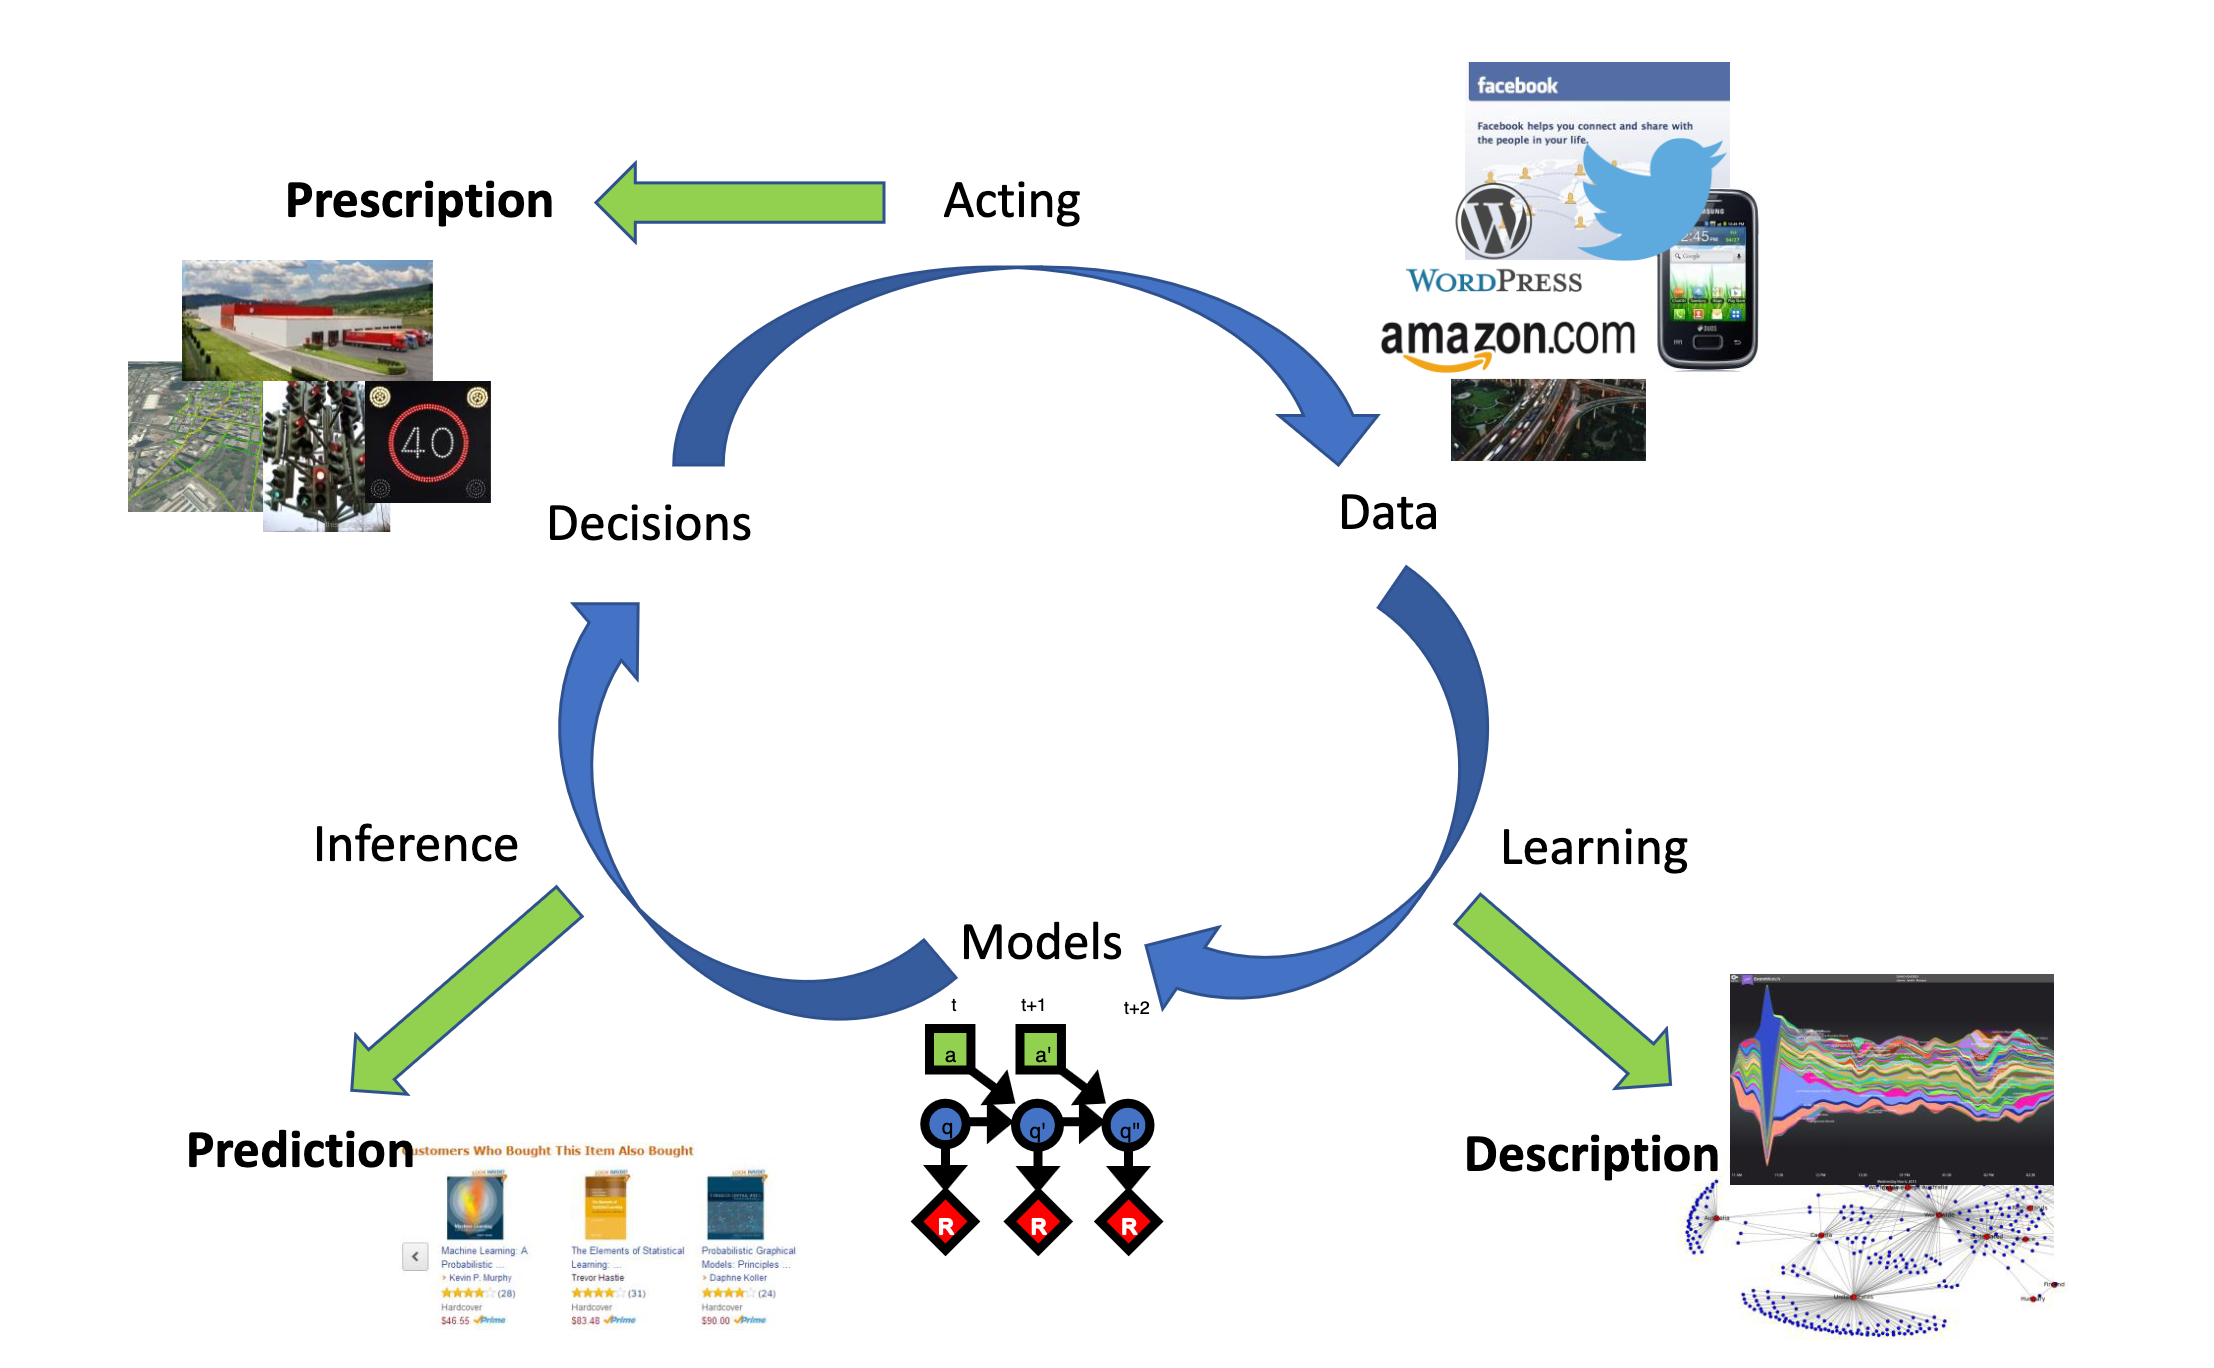
\includegraphics[width=\textwidth/2]{2.png}
\subsection{Data Science Hierarchy of Needs}
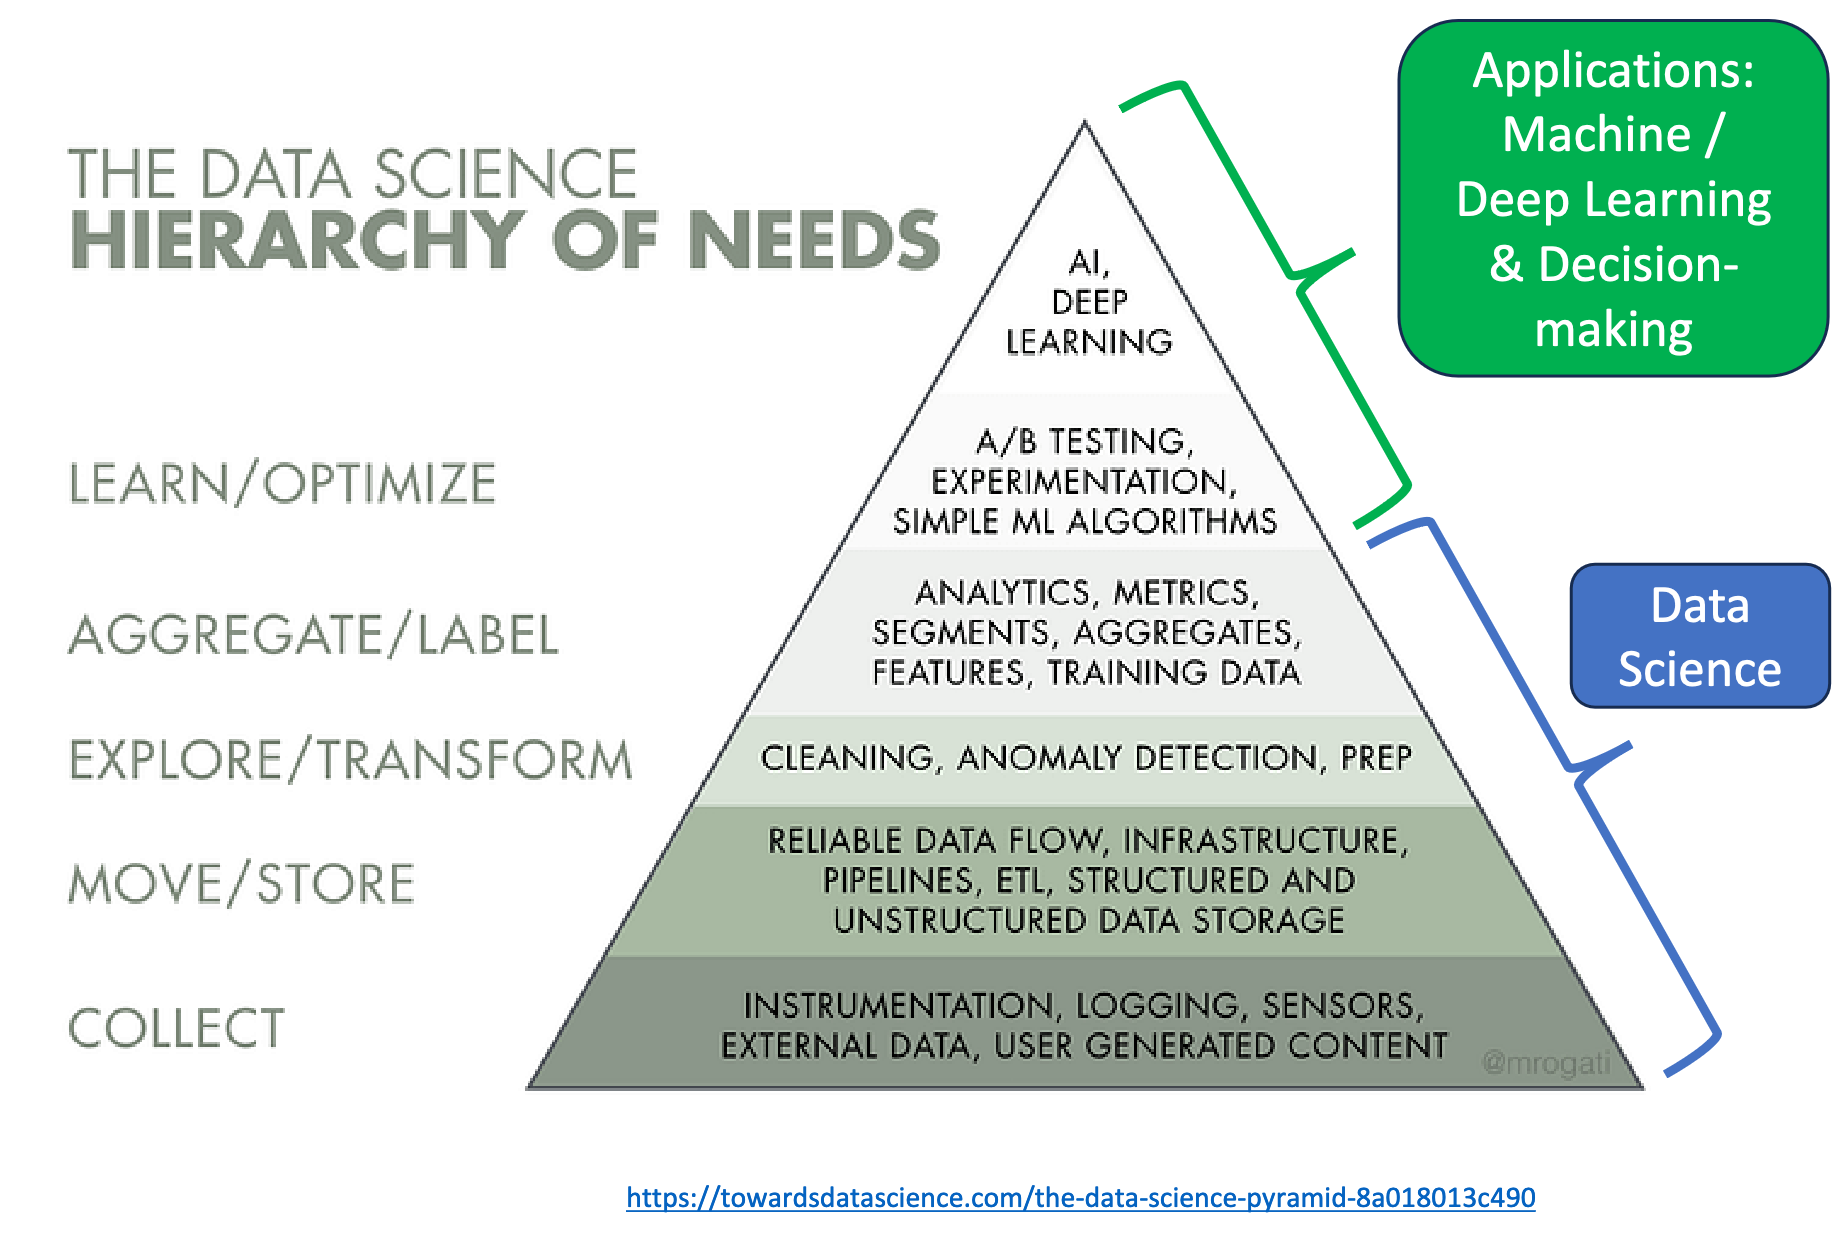
\includegraphics[width=\textwidth/2]{3.png}

\section{The Science of Data}
\subsection{Data are Observations of a Generative Process}
\begin{itemize}
  \item Data are the observables of a generative process
  \begin{itemize}
    \item We observe election votes of a population
    \item We observe Gallup poll survey of a population’s voting disposition
    \item Latent data generating process generated both
  \end{itemize}
  \item Example: 2016 US Presidential Election
  \begin{itemize}
    \item Gallup Poll Surveys predicted a landslide for Hillary Clinton
    \item We know how the election turned out
    \item Why was there a discrepancy?
    \begin{itemize}
      \item Sample bias in surveys
      \item Human behavioural biases in revealing their true preferences
    \end{itemize}
  \end{itemize}
  \item We care about the (latent) variables that generate the data
  \begin{itemize}
    \item We can use understanding of this generative process for prediction
    \item Aside: critically connected to modern perspective of Generative AI
  \end{itemize}
\end{itemize}
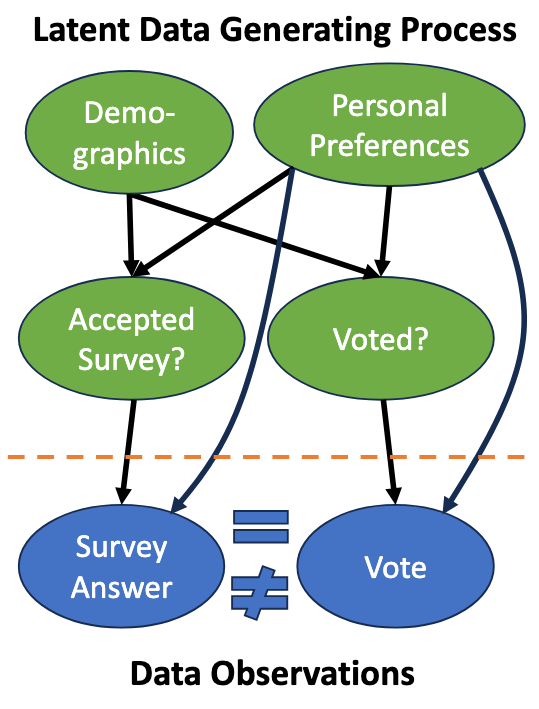
\includegraphics[scale = 0.25]{14.png}
% \begin{wrapfigure}{r}{0.25\textwidth} %this figure will be at the right
%   \centering
%   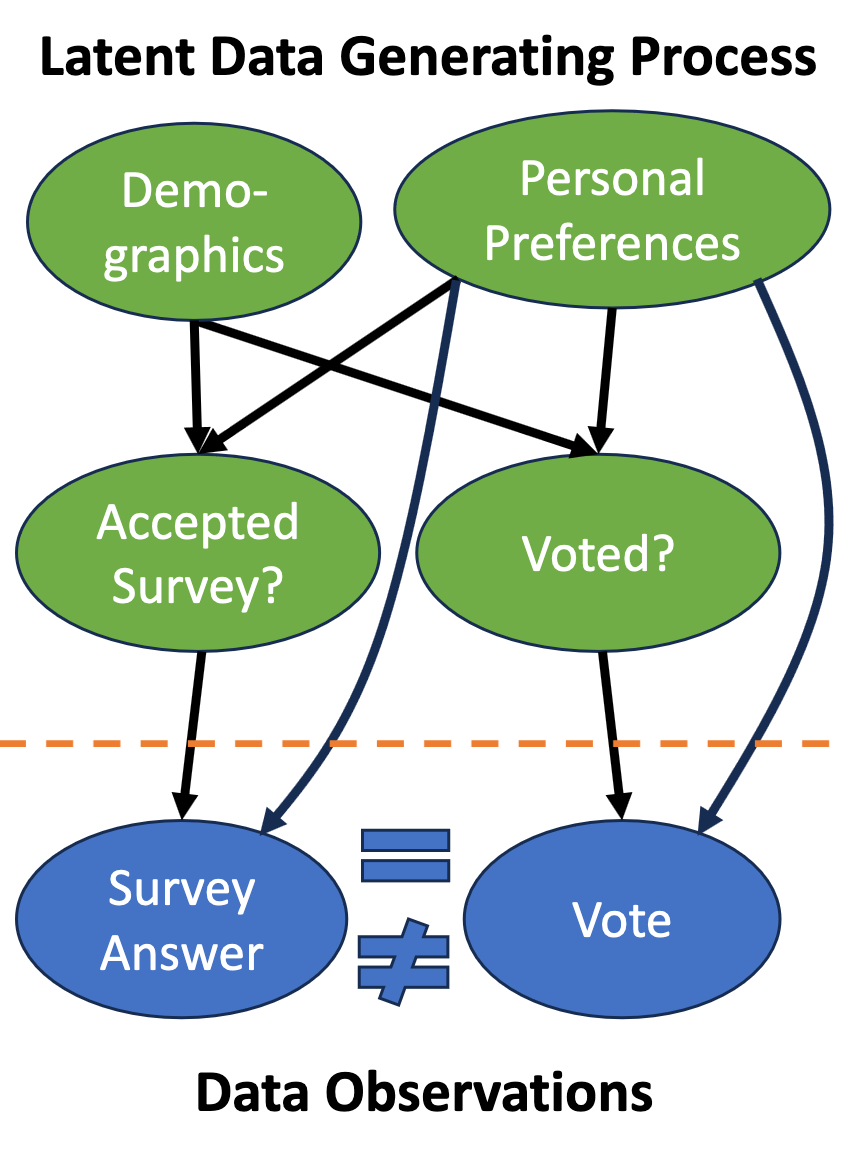
\includegraphics[width=0.25\textwidth]{4.png}
% \end{wrapfigure}

\subsection{Methodology of Data Science}
\begin{enumerate}
  \item Start: Real-world task or problem (business needs, societal or scientific problem)
  \begin{itemize}
    \item E.g, investigate sales performance, transit access and equity, pollution impacts on society
  \end{itemize}
  \item Develop research questions (RQs) and hypotheses
  \begin{itemize}
    \item Can we predict seasonal trends in perishable demands of food to reduce waste \& sales loss?
    \item Is public transit access equitably allocated among high and low income areas of a city?
    \item Does increased pollution lead to increased mortality rates?
  \end{itemize}
  \item Collect relevant data to test the hypotheses and answer the RQs
  \begin{itemize}
    \item Need to collect data or extract it from existing sources (Data Engineering, ETL)
    \item Need data for RQ that is representative of downstream use (performance, fairness \& bias)
  \end{itemize}
  \item Clean the data!
  \item Perform exploratory analysis on the data (feature analysis and visualization)
  \begin{itemize}
    \item Consider revisiting the data collection and cleaning process based on this data
  \end{itemize}
  \item Evaluate the original hypotheses and RQs w.r.t. the data, iterate as needed
  \item Finish: Report back to stakeholders (decision-making)
\end{enumerate}

\subsection{Data as a Science}
Data Science starts with a task and questions.
e.g. does increased pollution lead to higher mortality?
\begin{itemize}
  \item Data is a Science
  \begin{itemize}
    \item Science is the Scientific Method (the “why”)
    \item Engineering is the “how”
  \end{itemize}
  \item Recap: Scientific Method
  \begin{enumerate}
    \item Ask a Question
    \item Make a Falsifiable Hypothesis
    \item Design an Experiment to test the hypothesis
    \item If Hypothesis is falsified, go to step 2
  \end{enumerate}
  \item Be careful, details matter and many things can go wrong!
  \begin{itemize}
    \item E.g., statistical fallacies arise from multiple hypothesis testing
    \begin{itemize}
      \item The more datasets you compare, the more likely that two randomly correlate
      \item Can mitigate this with a Bonferroni Correction
    \end{itemize}
  \end{itemize}
\end{itemize}

\subsection{Spurious Correlations and Multiple Hypothesis Testing}
\begin{note}
  Spurious: comparing so many datapoints that it is bound to correlate. 
  Correlation is \textbf{not} conducive of causation.
\end{note}
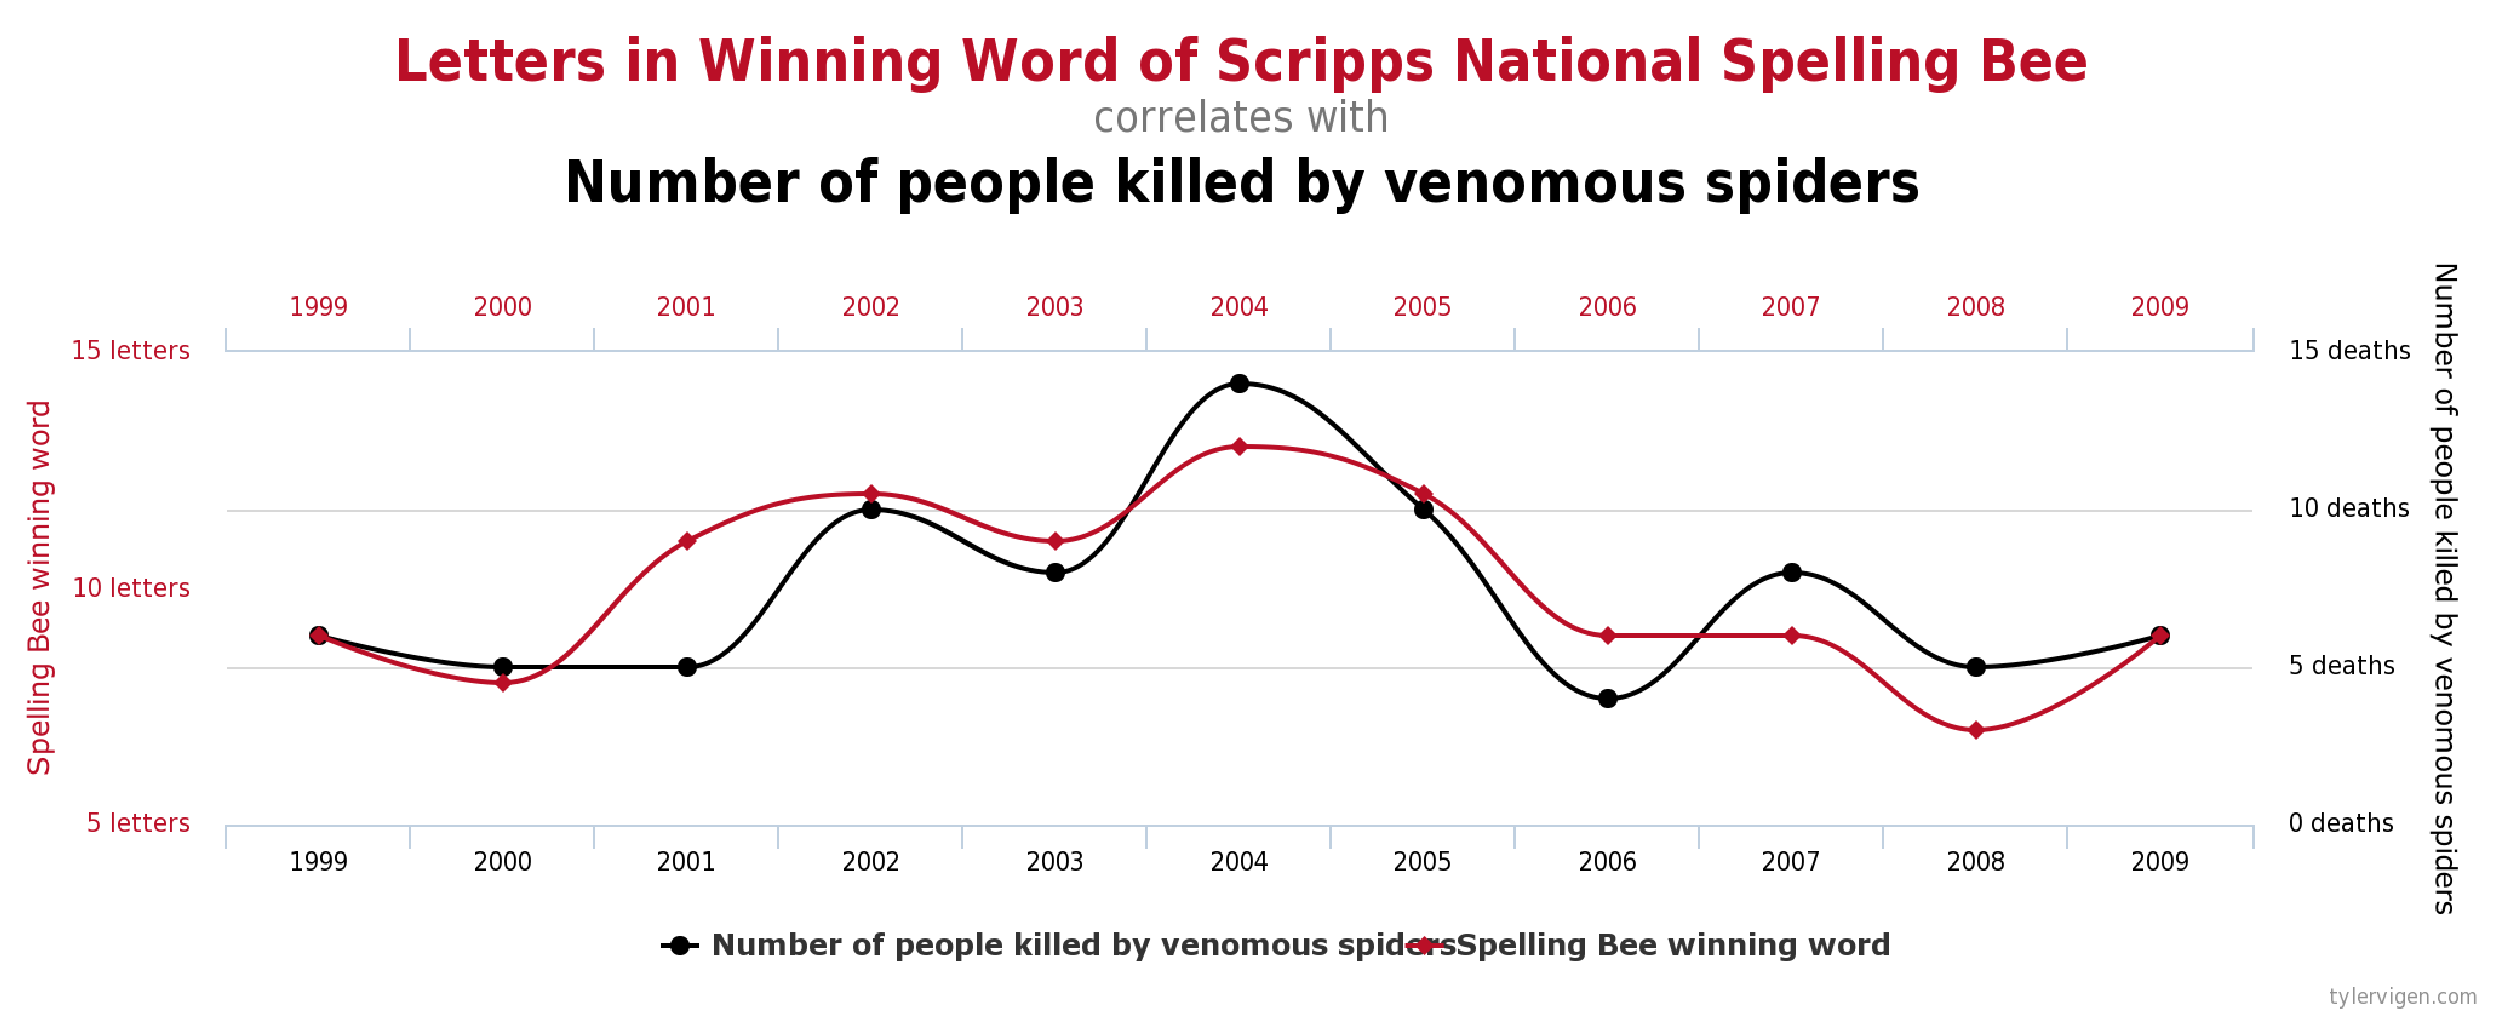
\includegraphics[width = \textwidth]{5.png}

\section{Data Comes in All Shapes and Forms}
Need proficiency in how to leverage structure of data and understanding of nuances of handling each data type
\subsection{Tabular Data (i.e., Pandas)}
\begin{note}
  NaN: Not a Number.
\end{note}
  \begin{itemize}
    \item Passengers on the Titanic
    \item 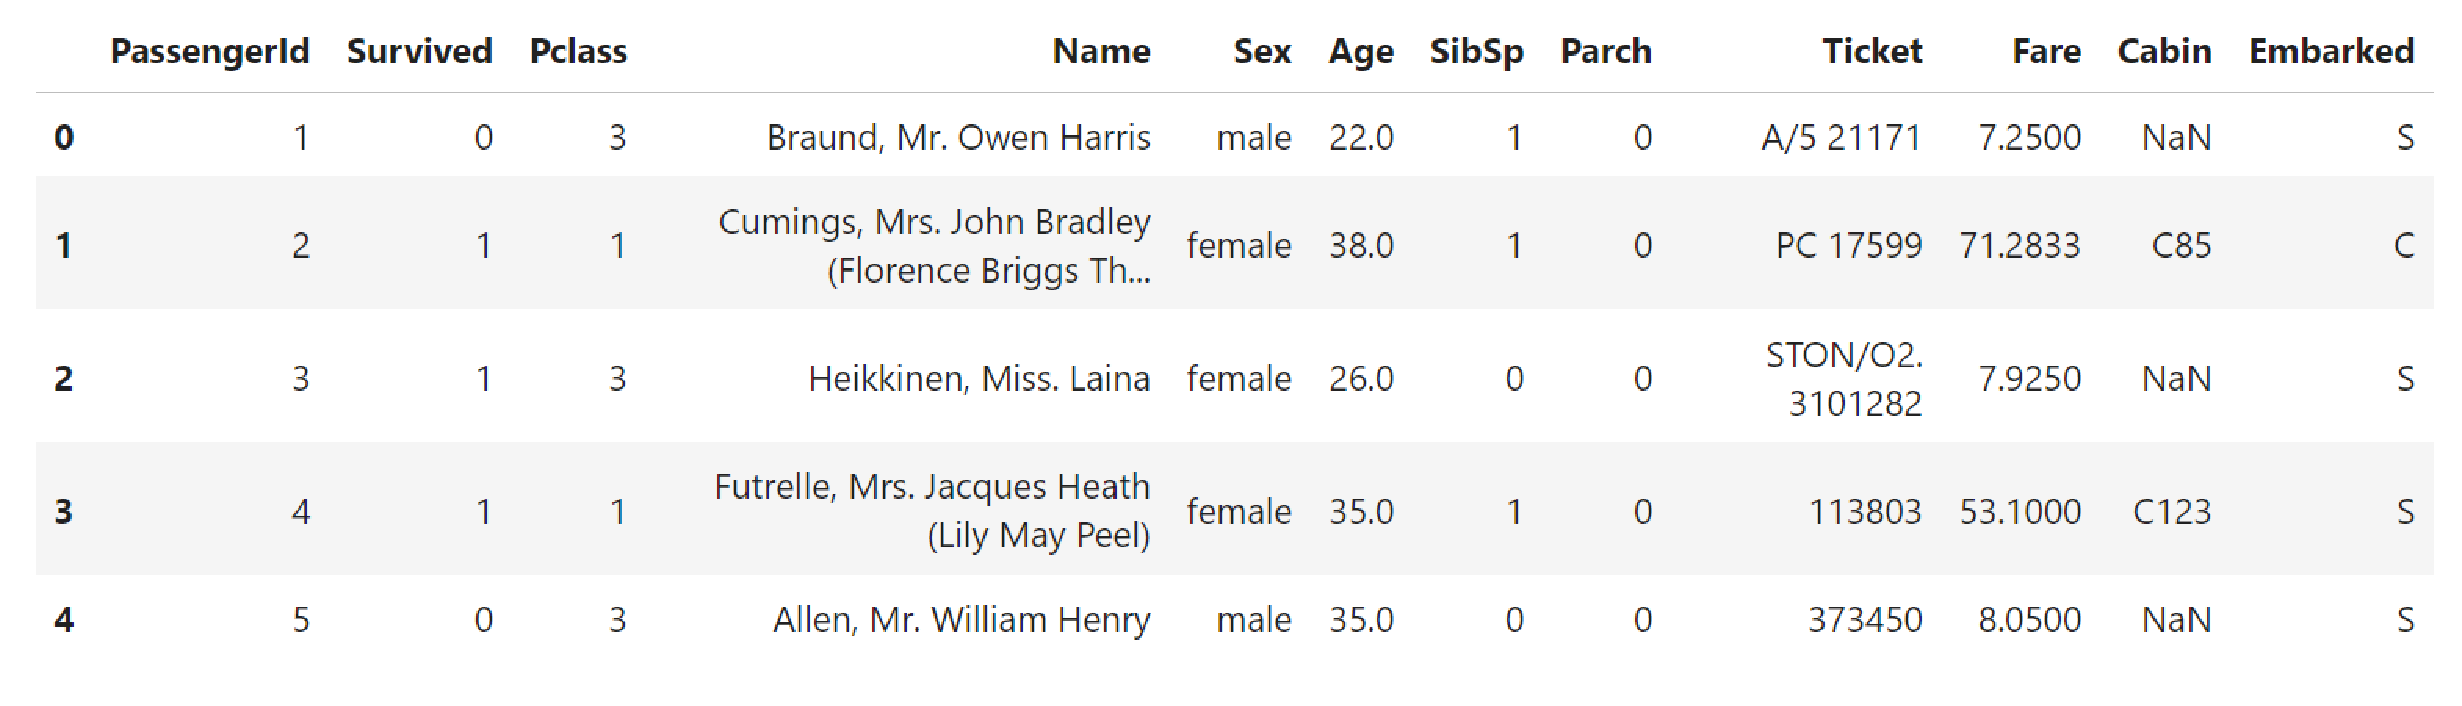
\includegraphics[width = \textwidth - 27.37506pt]{6.png}
  \end{itemize}
\subsection{Text Data and Analytics}
% \begin{wrapfigure}{r}{0.25\textwidth} %this figure will be at the right
%   \centering
%   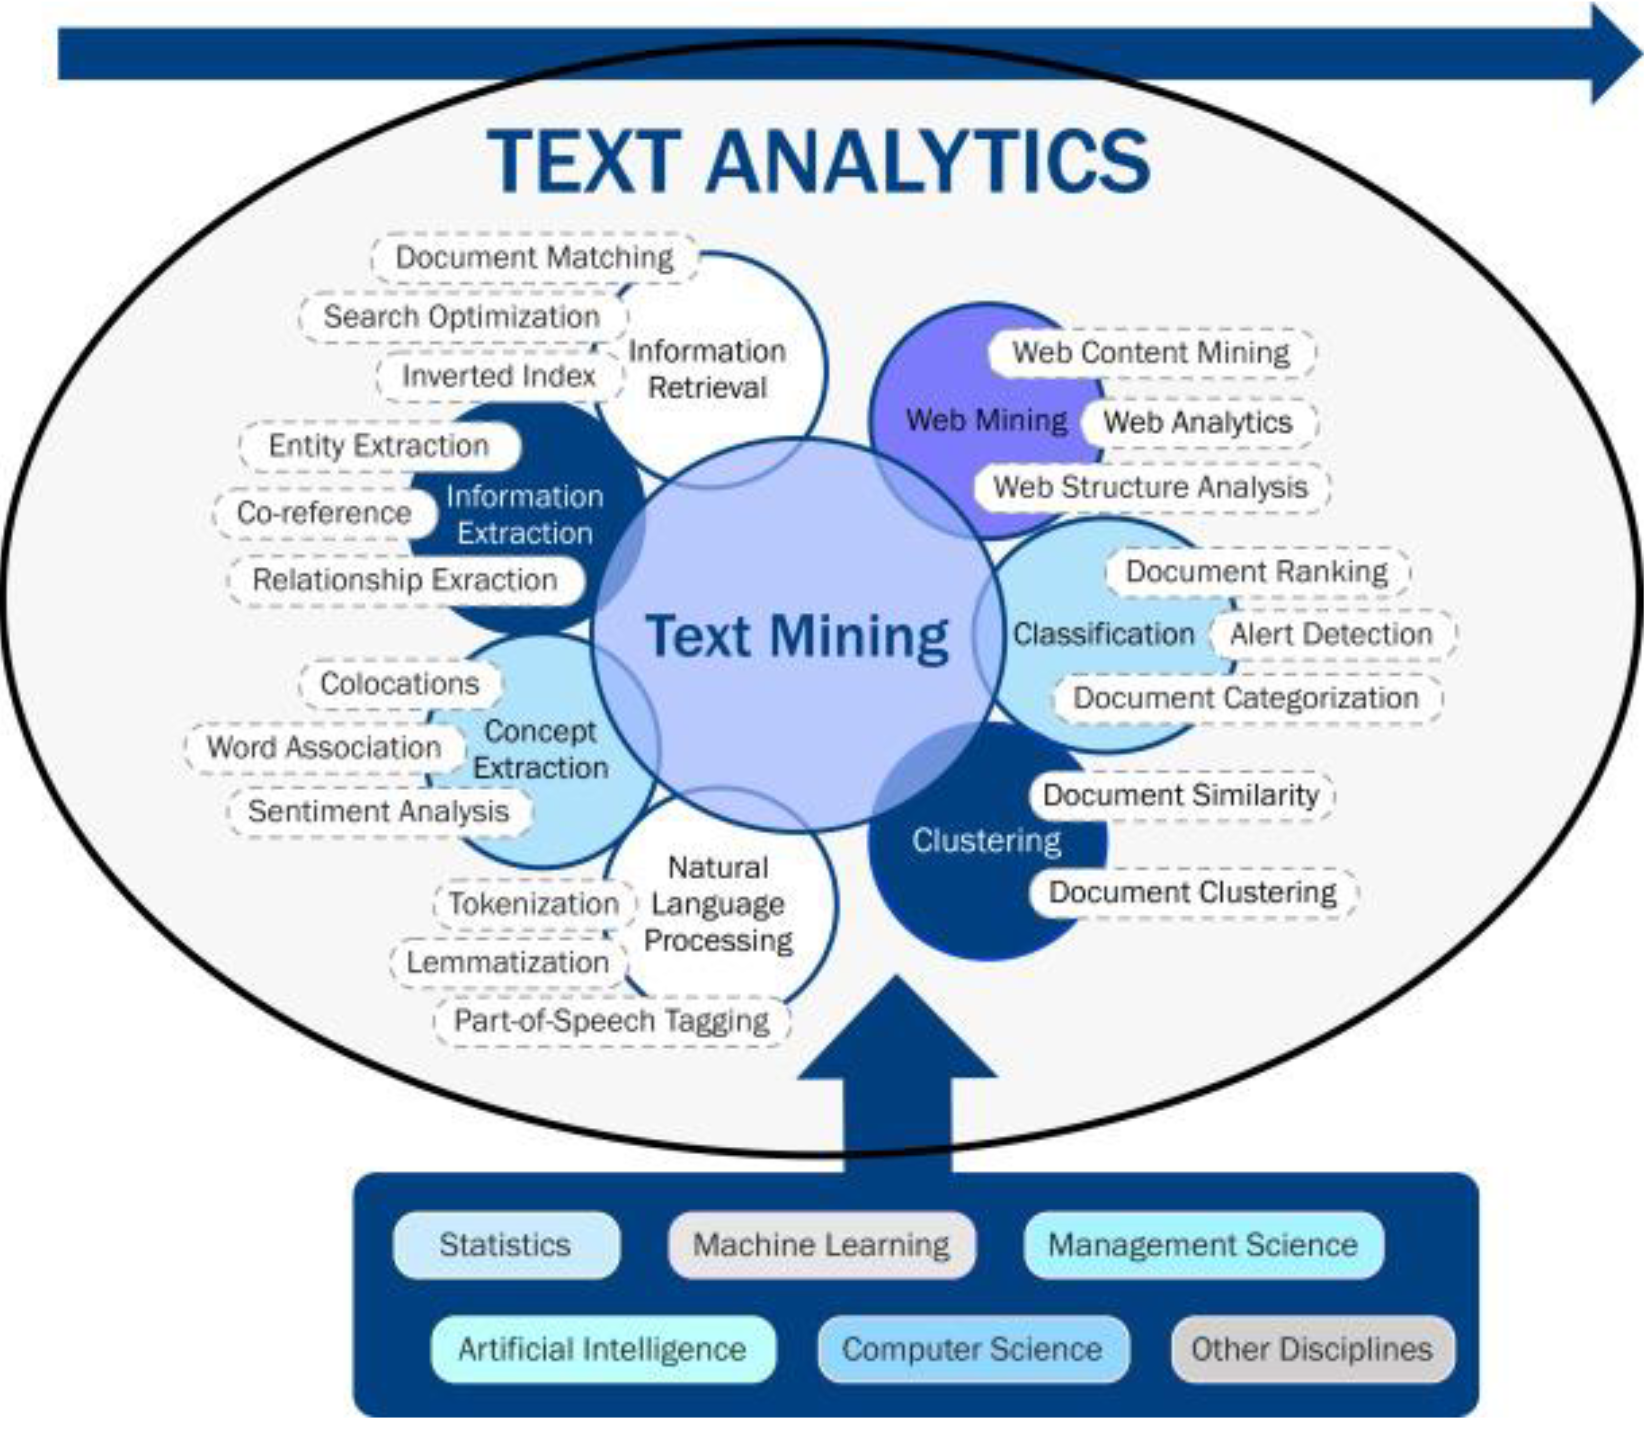
\includegraphics[width=0.25\textwidth]{13.png}
% \end{wrapfigure}
% \FloatBarrier
\begin{itemize}
  \item ~75\% of Data most IEs work with is text!
  \item Sources:
  \begin{itemize}
    \item Customer Feedback
    \item Reviews
    \item Blogs
    \item Social Media
    \item Academic Publication
    \item Healthcare / records
    \item News
  \end{itemize}
\end{itemize}
\subsection{Time Series Data}
Due to the famine and ex-immigration, the population in Ireland decreased while Europe's increased.
\begin{figure}
  \centering
  \begin{subfigure}{.5\textwidth}
    \centering
    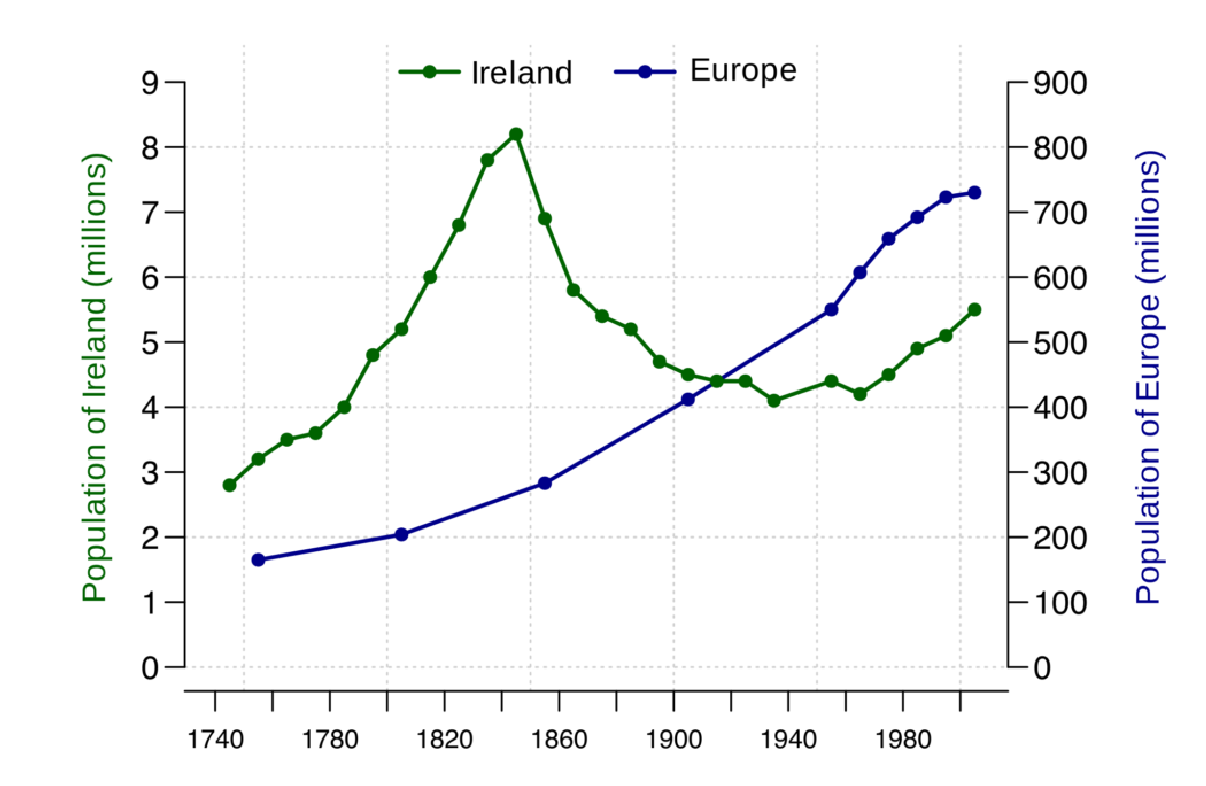
\includegraphics[width=.5\linewidth]{7.png}
    \caption{Population of Europe and Ireland vs. Year (1740-1990)}
    \label{fig:sub1}
  \end{subfigure}%
  \begin{subfigure}{.5\textwidth}
    \centering
    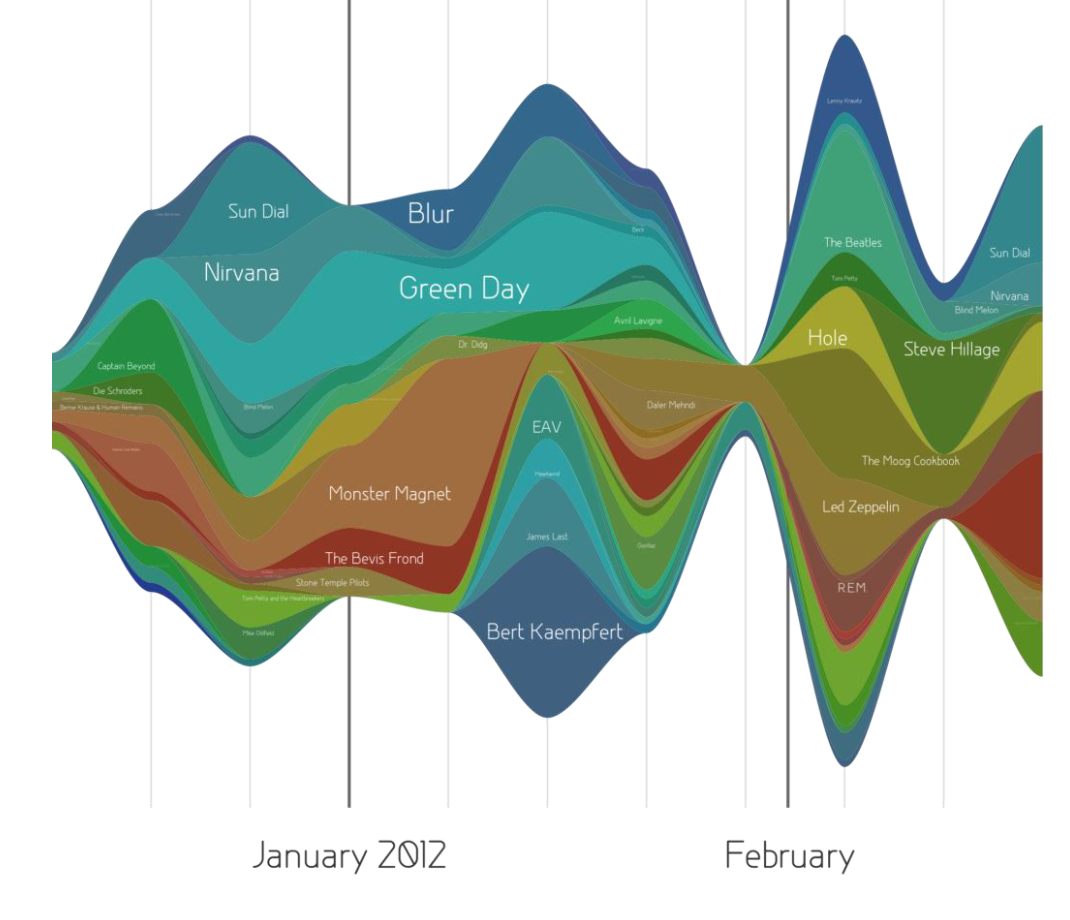
\includegraphics[width=.5\linewidth]{8.png}
    \caption{Stream Graph of a Last.fm user’s Time Spent Listening to Different Artists}
    \label{fig:sub2}
  \end{subfigure}
  \caption{Time Series Data}
  \label{fig:1}
\end{figure}
\FloatBarrier
\subsection{Network / Graph Data}
Communication is aligned with management structure.

Political blogs live in their own echo chambers.

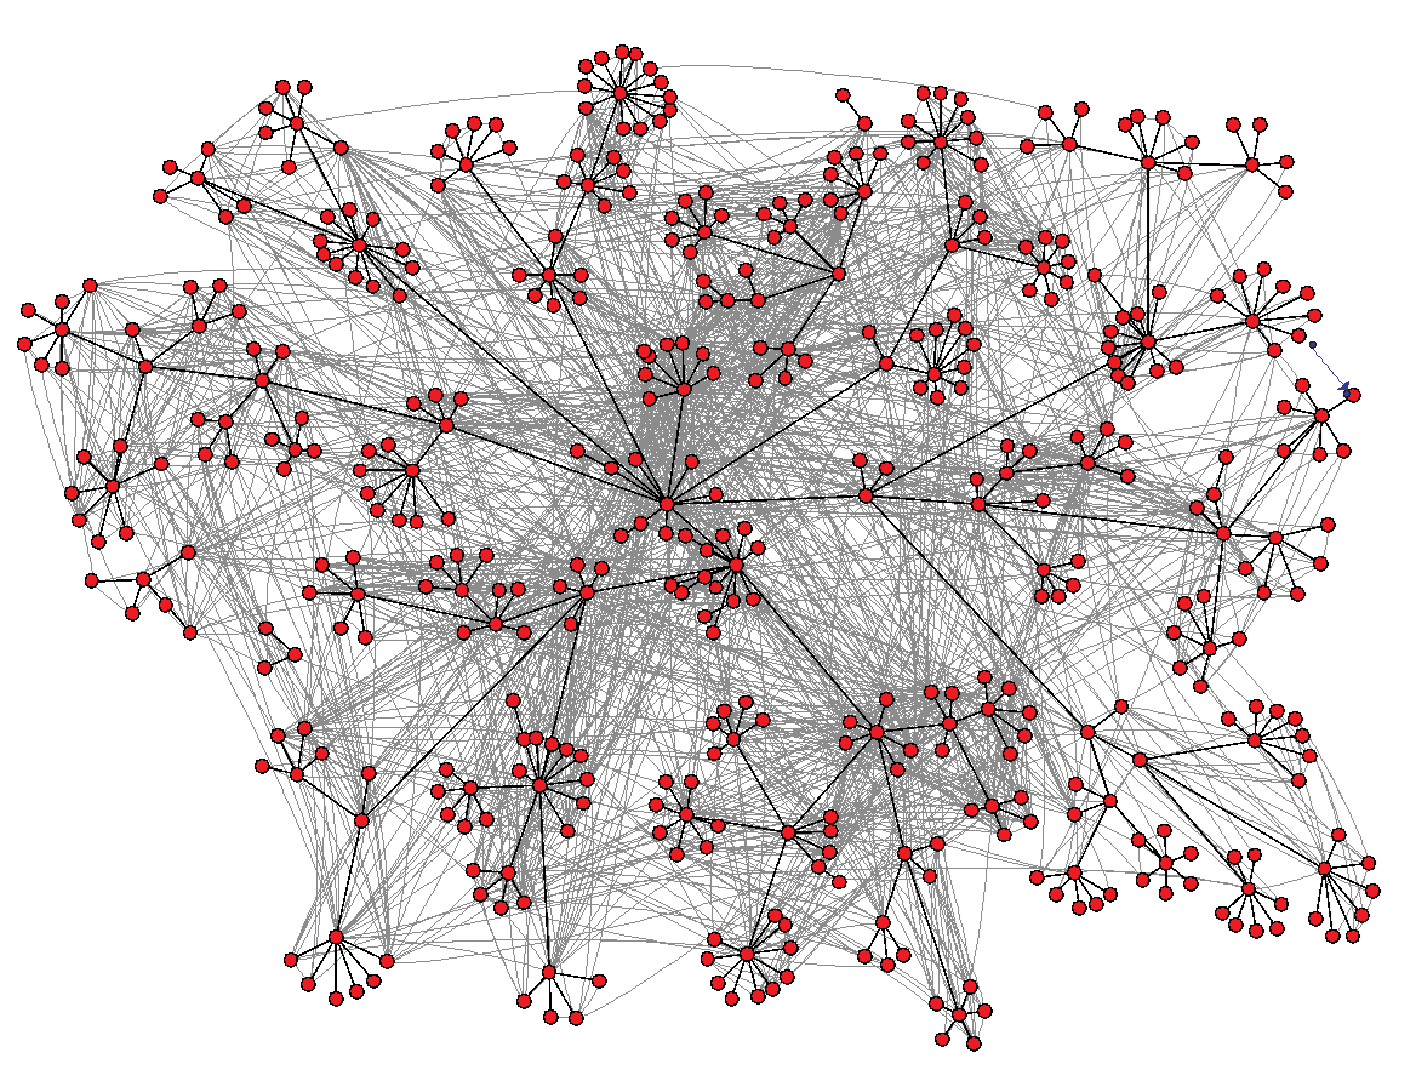
\includegraphics[width=.3\linewidth]{9.png}
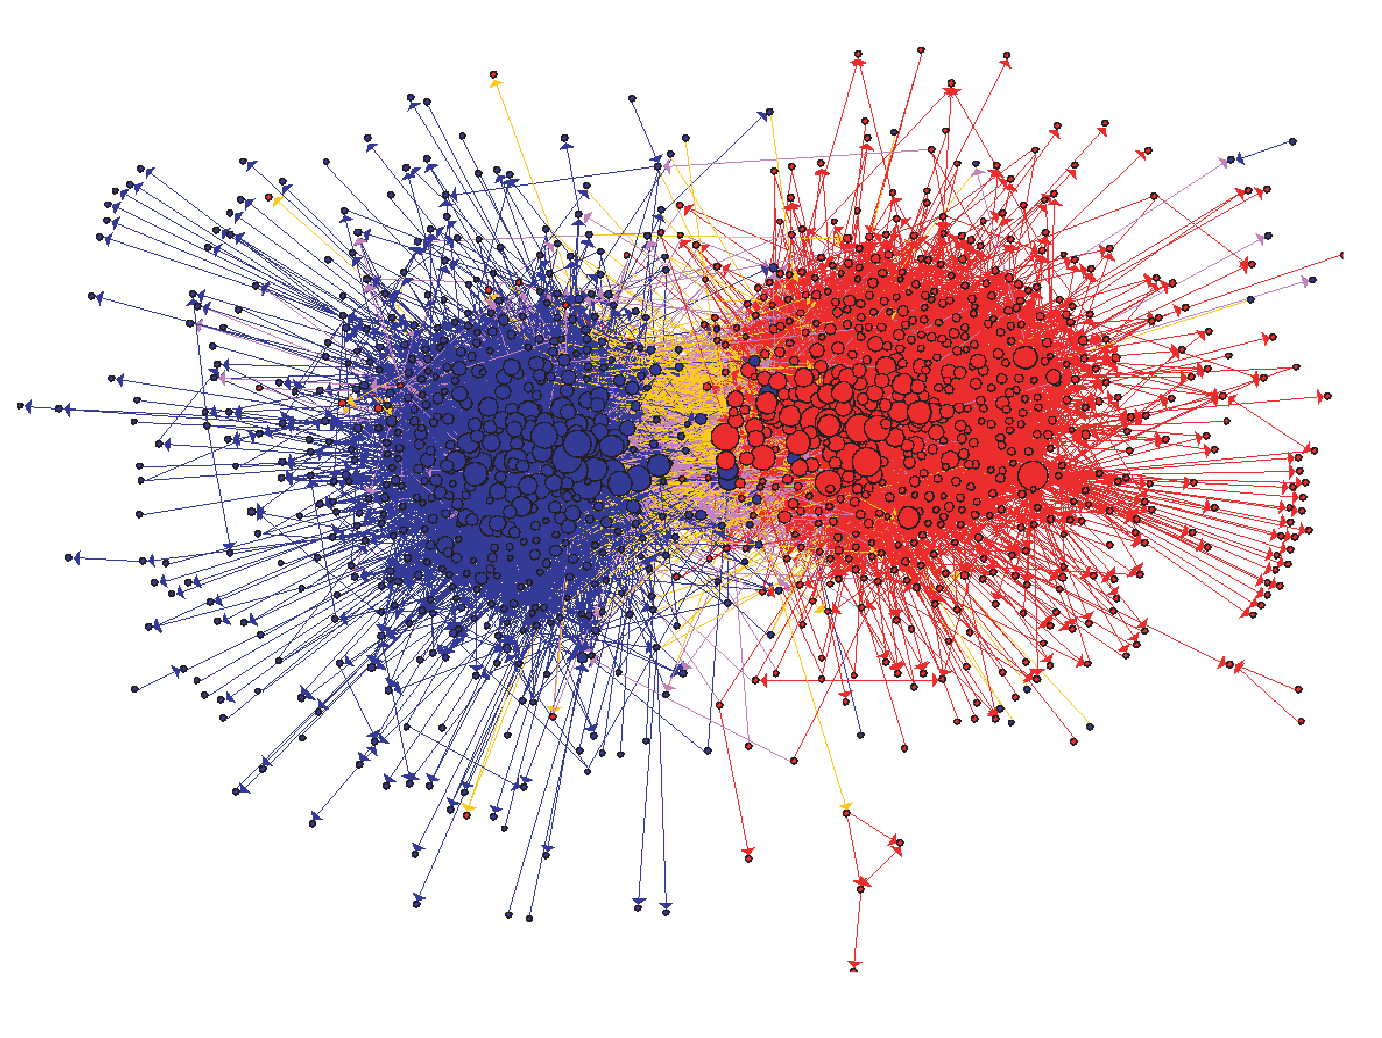
\includegraphics[width=.3\linewidth]{10.png}

% \begin{figure}
%   \centering
%   \begin{subfigure}{.5\textwidth}
%     \centering
%     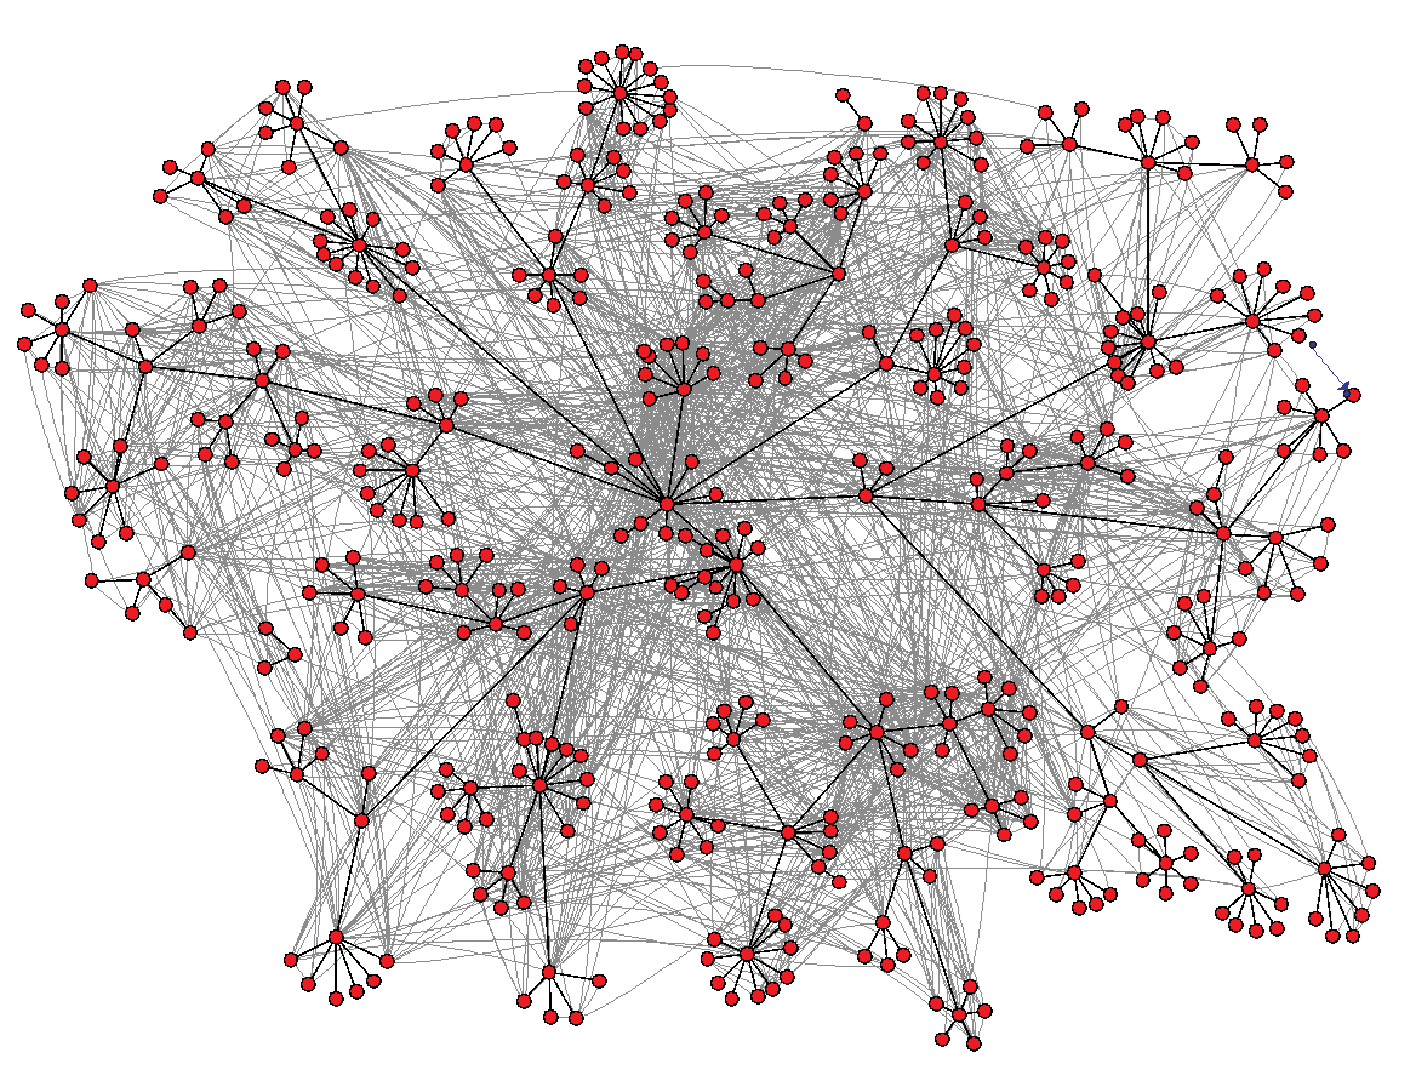
\includegraphics[width=.4\linewidth]{9.png}
%     \caption{HP Labs Manager and Email Network}
%     \label{fig:sub3}
%   \end{subfigure}
%   \begin{subfigure}{.5\textwidth}
%     \centering
%     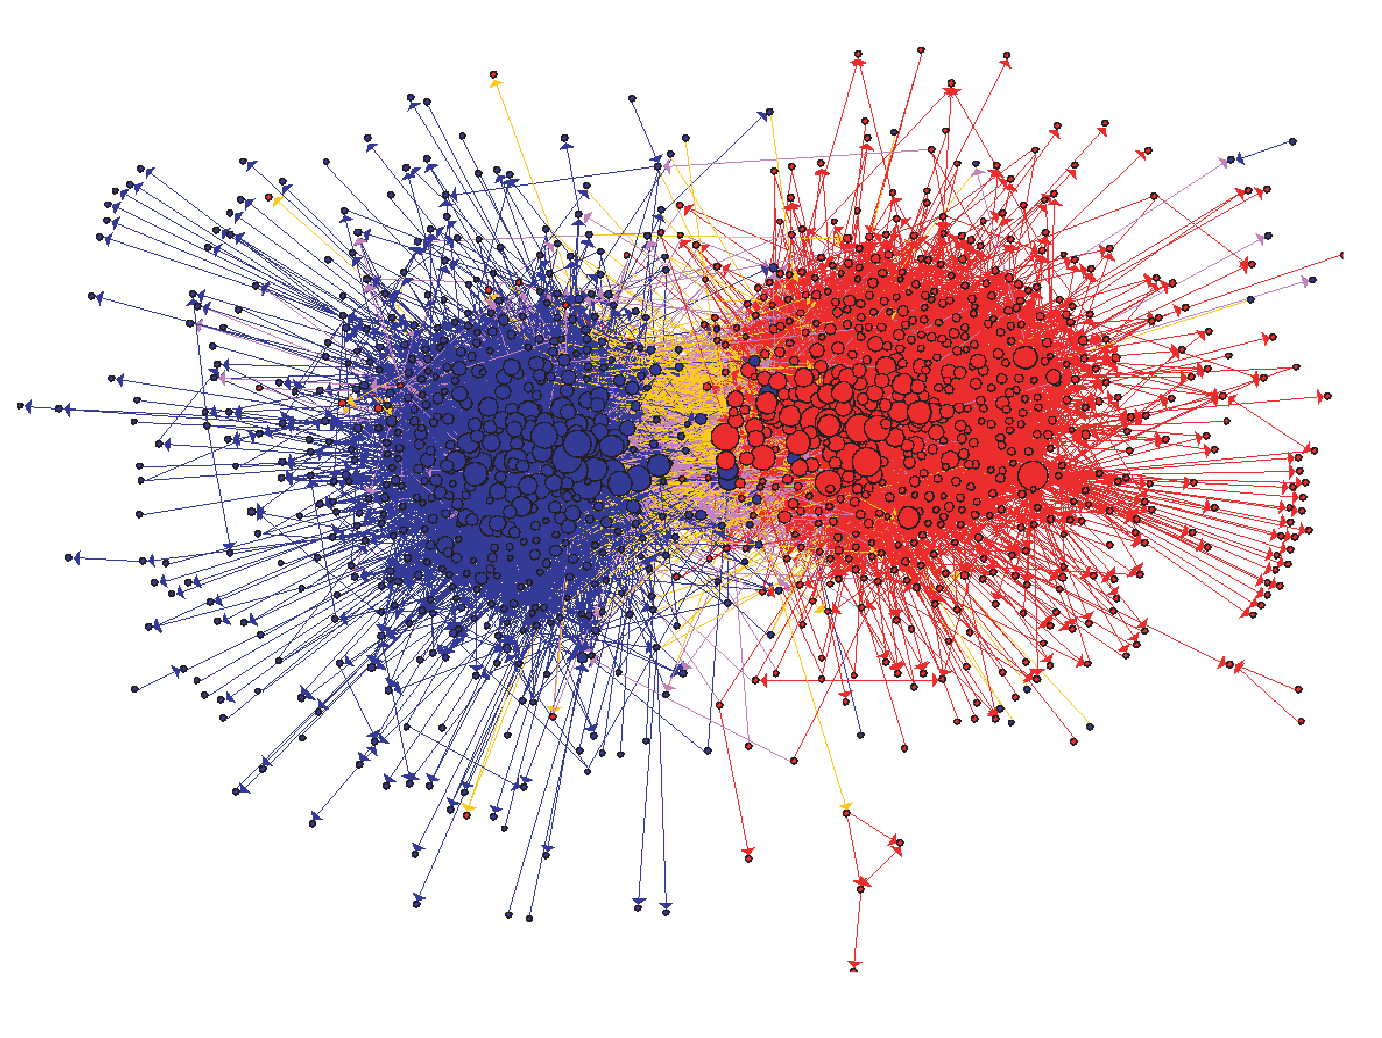
\includegraphics[width=.4\linewidth]{10.png}
%     \caption{Link Structure of Political Blogs}
%     \label{fig:sub4}
%   \end{subfigure}
%   \caption{Network / Graph Data}
%   \label{fig:2}
% \end{figure}
% \FloatBarrier
\subsection{Knowledge Graph Networks: Ingredients}
  Edges connect combined ingredients. 
  There becomes two main clusters of ingredients that are commonly used together.
  The two clusters are sweet and savoury ingredients.

  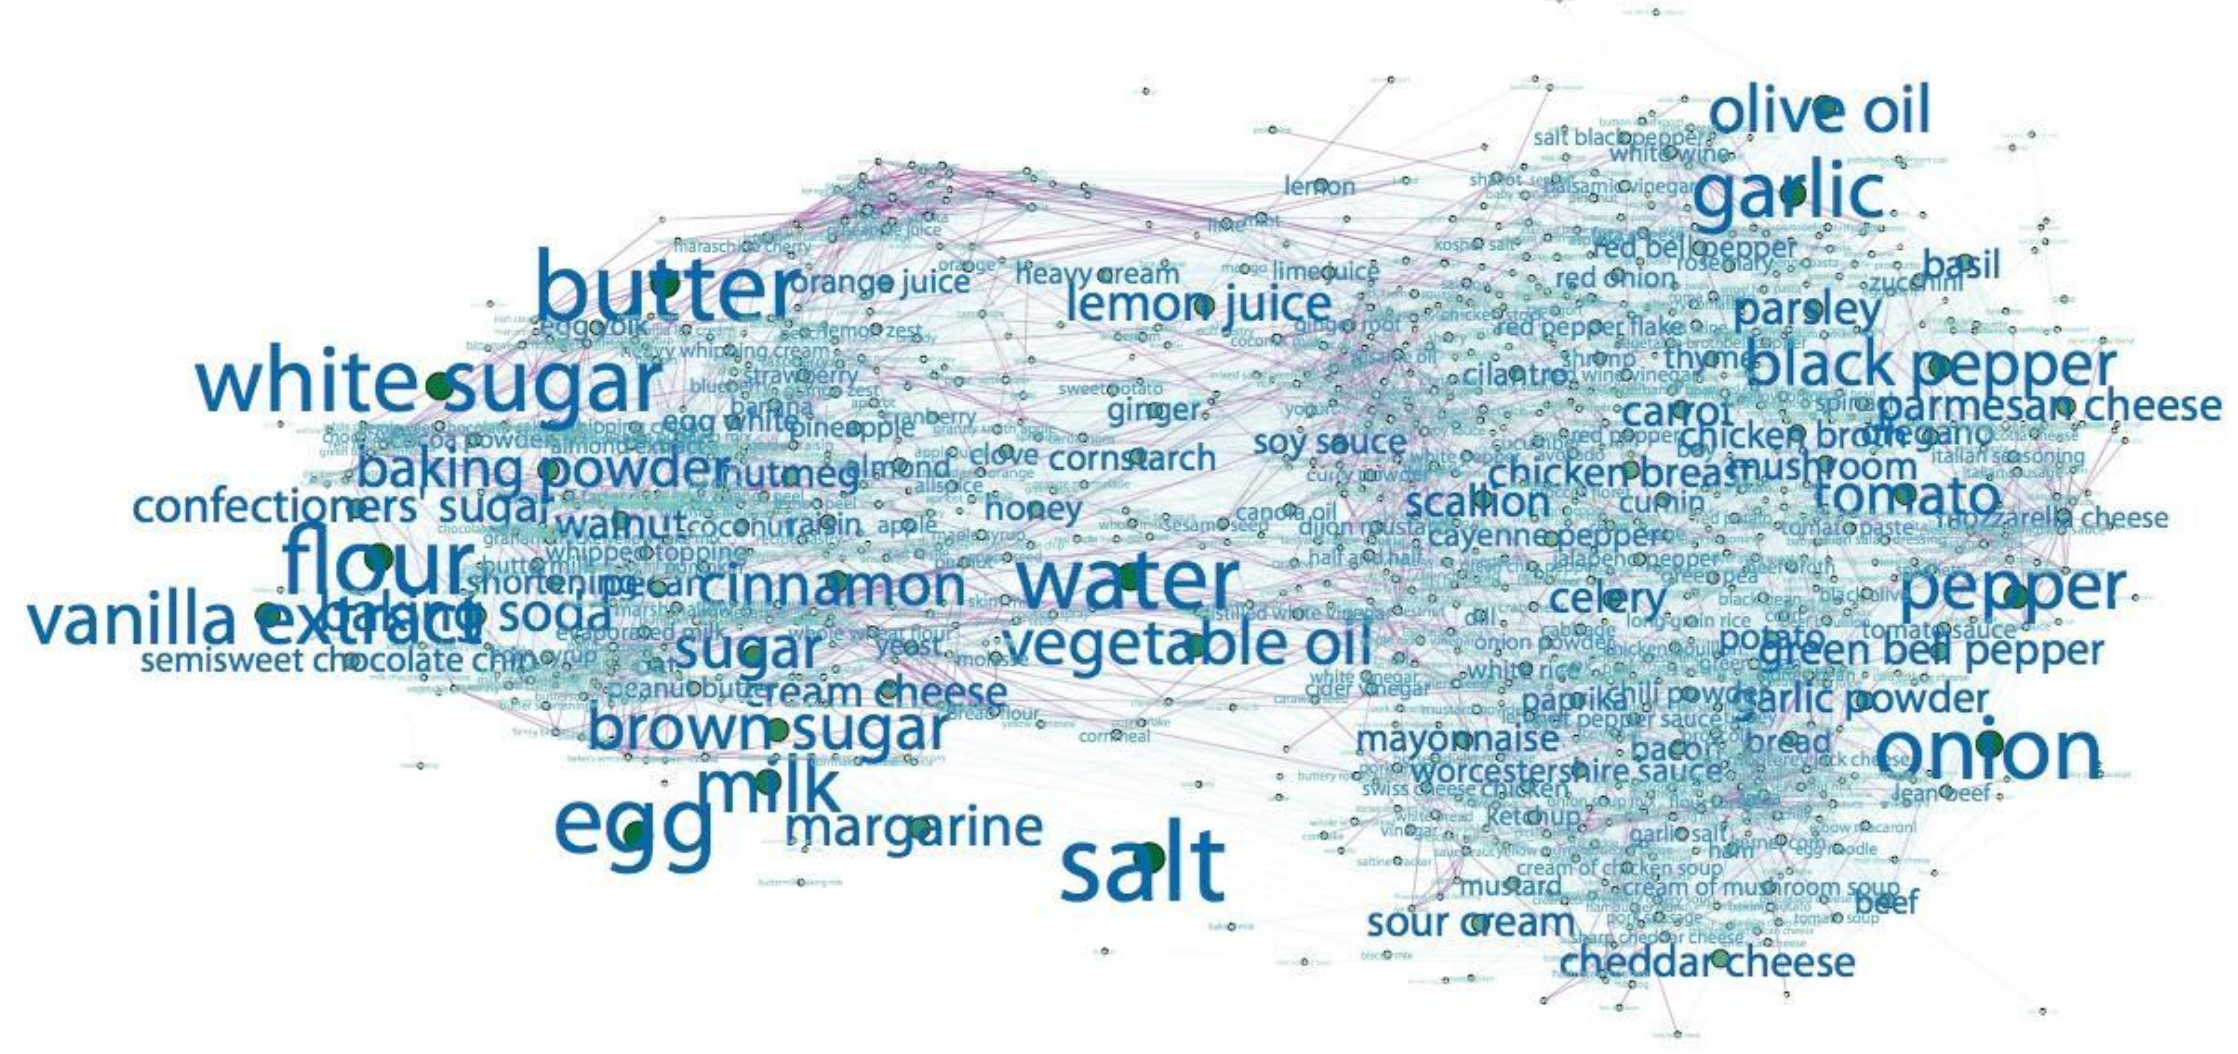
\includegraphics[width=\textwidth/2]{15.png}

\subsection{Geographical Data (Choropleths)}

  \begin{figure}[h]
    \centering
    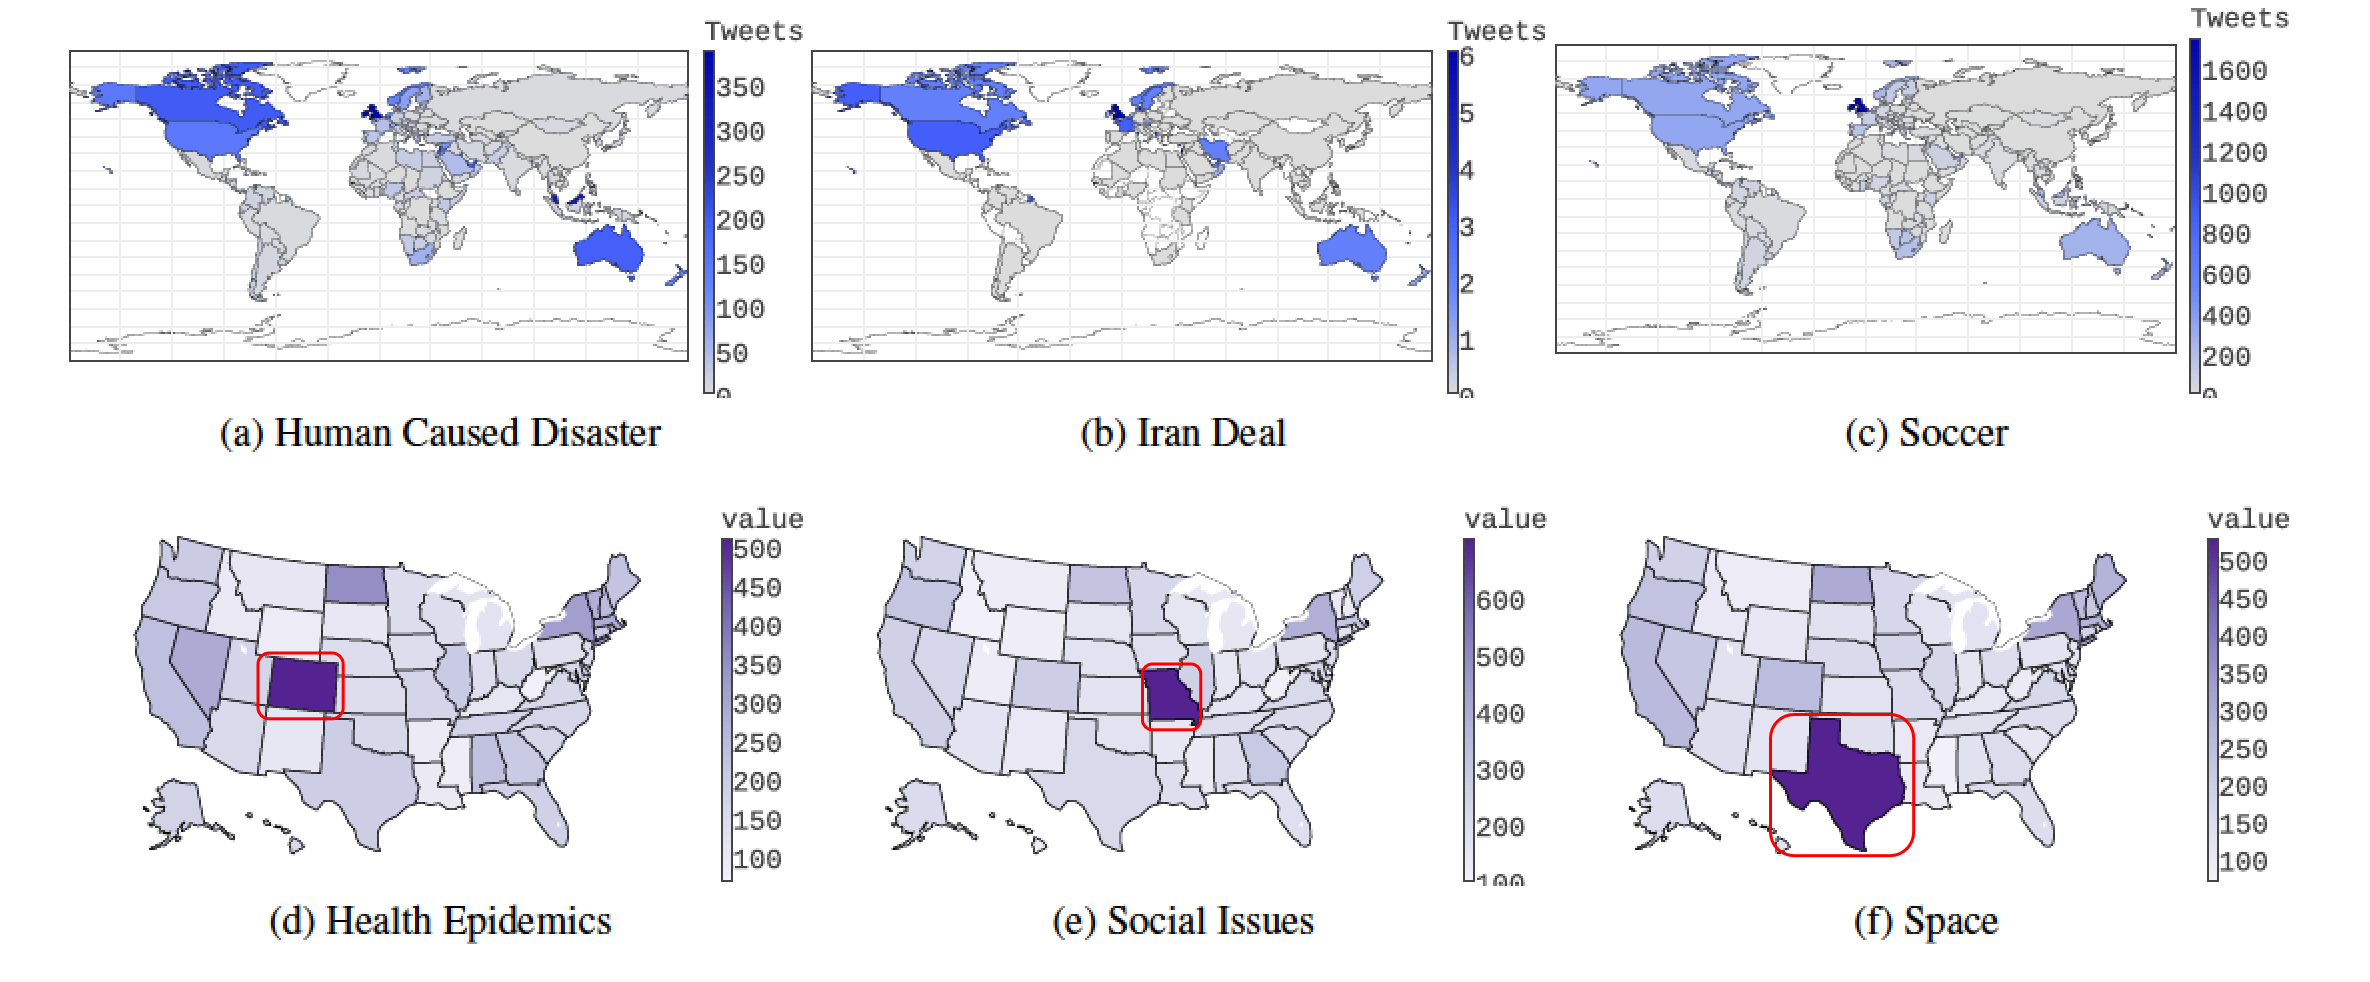
\includegraphics[width=\textwidth]{11.png}
    \caption{Per capita tweet (X) frequency across different international and U.S. locations for different topics}
    \label{fig:3}
  \end{figure}
\subsection{Geographical (GIS) Data}
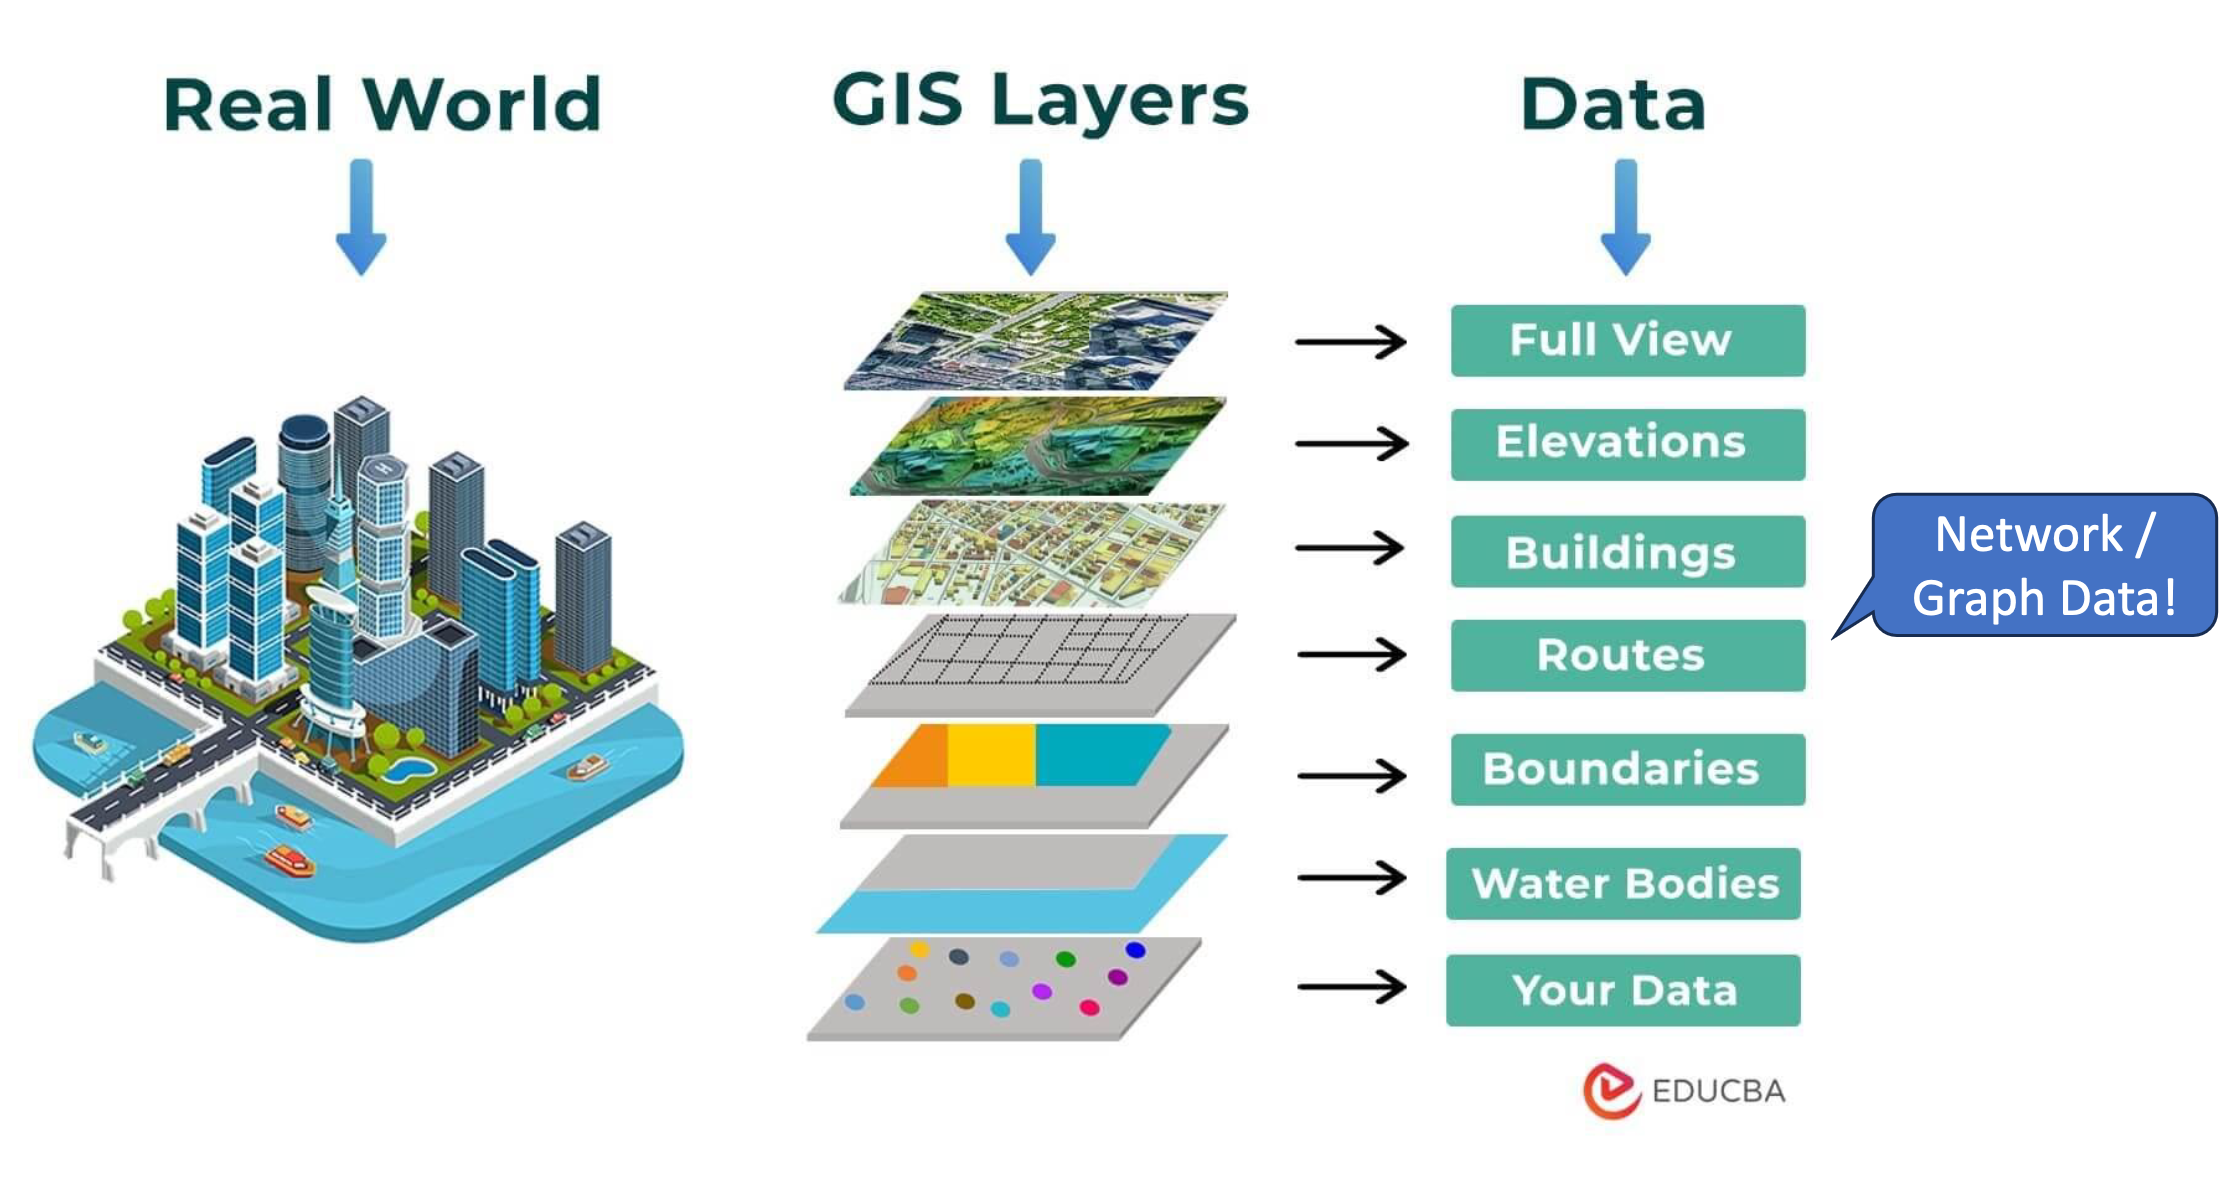
\includegraphics[width = \textwidth/2]{12.png}

\section{Content Highlights}
\subsection{Data Cleaning and Exploratory Data Analysis}
\begin{itemize}
  \item Data Cleaning
  \begin{itemize}
    \item Data summary
    \begin{itemize}
      \item Simple column analysis (basic statistics) and univariate visualization (histograms)
      \item Correcting (mixed) types, validating ranges, checking for outliers
    \end{itemize}
    \item Dealing with missing data
    \begin{itemize}
      \item Types of missingness, imputation
    \end{itemize}
    \item Data transformation
    \begin{itemize}
      \item Smoothing, aggregation, generalization, derived features, normalization (e.g. [min,max] or z-score)
    \end{itemize}
  \end{itemize}
  \item Exploratory Data Analysis
  \begin{itemize}
    \item Feature Analysis
    \begin{itemize}
      \item Correlation, (Pointwise) Mutual Information, Cross-Entropy
    \end{itemize}
    \item Visualization
    \begin{itemize}
      \item Visualizations for discrete and continuous data
      \item Visualizations for univariate (histogram), bivariate (e.g., scatterplot), and multivariate data (bubble plot)
      \item Custom and interactive visualization!
    \end{itemize}
  \end{itemize}
\end{itemize}

\subsection{Working with Structured Data}
\begin{note}
  PMI: Point-Wise Mutual Information is not an acronym, it is an initialism.
\end{note}
\begin{itemize}
  \item Text data and natural language processing
  \begin{itemize}
    \item The NLP pipeline and token processing
    \begin{itemize}
      \item Beyond tokens to phrases (easier to understand)
    \end{itemize}
    \item Sentiment (polarity and beyond!)
    \item The power of PMI!
  \end{itemize}
  \item Time series data
  \begin{itemize}
    \item Smoothing
    \item Autocorrelation and cross-correlation
  \end{itemize}
  \item Network data (Knowledge graph and social networks)
  \begin{itemize}
    \item Centrality measures
    \item Betweenness clustering
  \end{itemize}
  \item Geographical data
  \begin{itemize}
    \item Shapefiles and chloropleths
    \item Vector vs. raster data
    \item Coordinate Reference Systems
  \end{itemize}
\end{itemize}

\subsection{Data Science in Practice}
\begin{itemize}
  \item Advanced Data Science and Fallacies
  \begin{itemize}
    \item Be careful... a lot can go wrong!
  \end{itemize}
  \item Bayesian Data Science
  \begin{itemize}
    \item How do we model complex generative data processes
    \item And infer latent properties of those models (especially with “small” data)
  \end{itemize}
  \item Privacy and Anonymity
  \begin{itemize}
    \item Releasing data is help to society and business
    \item But we need to maintain privacy obligations for this data
  \end{itemize}
  \item Fairness and Bias (not tested)
  \begin{itemize}
    \item Data is biased
    \item How do we ensure fairness in the use of the data
    \item We cannot have it all, so we need to make our fairness (parity) decisions carefully
  \end{itemize}
\end{itemize}
\end{document}